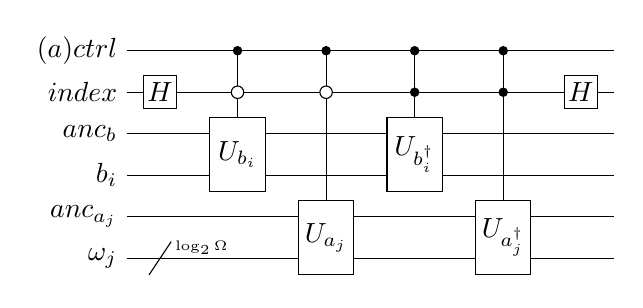
\begin{tikzpicture}[scale=1.000000,x=1pt,y=1pt]
\filldraw[color=white] (0.000000, -7.500000) rectangle (176.000000, 82.500000);
% Drawing wires
% Line 1: ctrl W \text{(a) }ctrl
\draw[color=black] (0.000000,75.000000) -- (176.000000,75.000000);
\draw[color=black] (0.000000,75.000000) node[left] {$\text{(a) }ctrl$};
% Line 2: index W index
\draw[color=black] (0.000000,60.000000) -- (176.000000,60.000000);
\draw[color=black] (0.000000,60.000000) node[left] {$index$};
% Line 3: anc_b W anc_b
\draw[color=black] (0.000000,45.000000) -- (176.000000,45.000000);
\draw[color=black] (0.000000,45.000000) node[left] {$anc_b$};
% Line 4: i W b_i
\draw[color=black] (0.000000,30.000000) -- (176.000000,30.000000);
\draw[color=black] (0.000000,30.000000) node[left] {$b_i$};
% Line 5: anc_a W anc_{a_j}
\draw[color=black] (0.000000,15.000000) -- (176.000000,15.000000);
\draw[color=black] (0.000000,15.000000) node[left] {$anc_{a_j}$};
% Line 6: j W \omega_j
\draw[color=black] (0.000000,0.000000) -- (176.000000,0.000000);
\draw[color=black] (0.000000,0.000000) node[left] {$\omega_j$};
% Done with wires; drawing gates
% Line 8: j / ^{\log_2{\Omega}}
\draw (8.000000, -6.000000) -- (16.000000, 6.000000);
\draw (14.000000, 3.000000) node[right] {$\scriptstyle{^{\log_2{\Omega}}}$};
% Line 10: index G $H$
\begin{scope}
\draw[fill=white] (12.000000, 60.000000) +(-45.000000:8.485281pt and 8.485281pt) -- +(45.000000:8.485281pt and 8.485281pt) -- +(135.000000:8.485281pt and 8.485281pt) -- +(225.000000:8.485281pt and 8.485281pt) -- cycle;
\clip (12.000000, 60.000000) +(-45.000000:8.485281pt and 8.485281pt) -- +(45.000000:8.485281pt and 8.485281pt) -- +(135.000000:8.485281pt and 8.485281pt) -- +(225.000000:8.485281pt and 8.485281pt) -- cycle;
\draw (12.000000, 60.000000) node {$H$};
\end{scope}
% Line 11: i anc_b G width=20 $U_{b_i}$ ctrl -index
\draw (40.000000,75.000000) -- (40.000000,30.000000);
\begin{scope}
\draw[fill=white] (40.000000, 37.500000) +(-45.000000:14.142136pt and 19.091883pt) -- +(45.000000:14.142136pt and 19.091883pt) -- +(135.000000:14.142136pt and 19.091883pt) -- +(225.000000:14.142136pt and 19.091883pt) -- cycle;
\clip (40.000000, 37.500000) +(-45.000000:14.142136pt and 19.091883pt) -- +(45.000000:14.142136pt and 19.091883pt) -- +(135.000000:14.142136pt and 19.091883pt) -- +(225.000000:14.142136pt and 19.091883pt) -- cycle;
\draw (40.000000, 37.500000) node {$U_{b_i}$};
\end{scope}
\filldraw (40.000000, 75.000000) circle(1.500000pt);
\draw[fill=white] (40.000000, 60.000000) circle(2.250000pt);
% Line 12: j anc_a G width=20 $U_{a_j}$ ctrl -index
\draw (72.000000,75.000000) -- (72.000000,0.000000);
\begin{scope}
\draw[fill=white] (72.000000, 7.500000) +(-45.000000:14.142136pt and 19.091883pt) -- +(45.000000:14.142136pt and 19.091883pt) -- +(135.000000:14.142136pt and 19.091883pt) -- +(225.000000:14.142136pt and 19.091883pt) -- cycle;
\clip (72.000000, 7.500000) +(-45.000000:14.142136pt and 19.091883pt) -- +(45.000000:14.142136pt and 19.091883pt) -- +(135.000000:14.142136pt and 19.091883pt) -- +(225.000000:14.142136pt and 19.091883pt) -- cycle;
\draw (72.000000, 7.500000) node {$U_{a_j}$};
\end{scope}
\filldraw (72.000000, 75.000000) circle(1.500000pt);
\draw[fill=white] (72.000000, 60.000000) circle(2.250000pt);
% Line 13: i anc_b G width=20 $U_{b_i^\dagger}$ ctrl index
\draw (104.000000,75.000000) -- (104.000000,30.000000);
\begin{scope}
\draw[fill=white] (104.000000, 37.500000) +(-45.000000:14.142136pt and 19.091883pt) -- +(45.000000:14.142136pt and 19.091883pt) -- +(135.000000:14.142136pt and 19.091883pt) -- +(225.000000:14.142136pt and 19.091883pt) -- cycle;
\clip (104.000000, 37.500000) +(-45.000000:14.142136pt and 19.091883pt) -- +(45.000000:14.142136pt and 19.091883pt) -- +(135.000000:14.142136pt and 19.091883pt) -- +(225.000000:14.142136pt and 19.091883pt) -- cycle;
\draw (104.000000, 37.500000) node {$U_{b_i^\dagger}$};
\end{scope}
\filldraw (104.000000, 75.000000) circle(1.500000pt);
\filldraw (104.000000, 60.000000) circle(1.500000pt);
% Line 14: j anc_a G width=20 $U_{a_j^\dagger}$ ctrl index
\draw (136.000000,75.000000) -- (136.000000,0.000000);
\begin{scope}
\draw[fill=white] (136.000000, 7.500000) +(-45.000000:14.142136pt and 19.091883pt) -- +(45.000000:14.142136pt and 19.091883pt) -- +(135.000000:14.142136pt and 19.091883pt) -- +(225.000000:14.142136pt and 19.091883pt) -- cycle;
\clip (136.000000, 7.500000) +(-45.000000:14.142136pt and 19.091883pt) -- +(45.000000:14.142136pt and 19.091883pt) -- +(135.000000:14.142136pt and 19.091883pt) -- +(225.000000:14.142136pt and 19.091883pt) -- cycle;
\draw (136.000000, 7.500000) node {$U_{a_j^\dagger}$};
\end{scope}
\filldraw (136.000000, 75.000000) circle(1.500000pt);
\filldraw (136.000000, 60.000000) circle(1.500000pt);
% Line 15: index G $H$
\begin{scope}
\draw[fill=white] (164.000000, 60.000000) +(-45.000000:8.485281pt and 8.485281pt) -- +(45.000000:8.485281pt and 8.485281pt) -- +(135.000000:8.485281pt and 8.485281pt) -- +(225.000000:8.485281pt and 8.485281pt) -- cycle;
\clip (164.000000, 60.000000) +(-45.000000:8.485281pt and 8.485281pt) -- +(45.000000:8.485281pt and 8.485281pt) -- +(135.000000:8.485281pt and 8.485281pt) -- +(225.000000:8.485281pt and 8.485281pt) -- cycle;
\draw (164.000000, 60.000000) node {$H$};
\end{scope}
% Done with gates; drawing ending labels
% Done with ending labels; drawing cut lines and comments
% Done with comments
\end{tikzpicture}
